\chapter{Technische Implementierung}

\section{Vorwort - technische Implementierung}
Als technische Grundlage für moosr wird ein Webframework verwendet, da dieses an
die benötigten Bedürfnisse (Suchmaschine) am relativ gut angepasst werden kann.
\\
Als Webframework haben wir uns mit Absprache mit Herrn Dr. Alois
Kastner-Maresch auf das Python Microwebframework Flask geeinigt da wir das
Framework in der Vorlesung \emph{Wiederverwendungsbasierte Entwicklung von
Systemen} in einer Studienarbeit erarbeiteten und das dort gewonnene Wissen (Flask
und Python) praktisch in der Vorlesung ,,Webtechnologie und Webmarketing 
mit Open Source'' umsetzen möchten.

\section{Verwendete Frameworks}

\subsection{Flask}
Das Microwebframework benutzt \emph{Jinja} als Template Renderengine und
\emph{Werkzeugs} als WSGI Middleware. Die Pakete selbst können mit pip gezogen
werden.
\\
Da die Webpräsentation primär als Dienstleistung zu sehen ist kommen bei der
Implementierung neben dem Framework selbst hauptsächlich auf die beiden
libraries \emph{libglyr} und \emph{sqlite3} zum Einsatz.

\subsection{libglyr}
Libglyr ist eine library zum auffinden von Musikmetadaten. 
\\
\begin{center}
\url{https://github.com/sahib/glyr}
\end{center}

\subsection{sqlite3}
Sqlite3 ist eine sehr weit genutzte und bekannte embedded Datenbank, welche für
unseren Einsatz optimal ist.
\\
\begin{center}
\url{http://www.sqlite.org/}
\end{center}


\section{Historisches}

Wie bereits erwähnt ging die aktuelle Seite aus einer Studienarbeit im Fach 
,,Wiederverwendungsbasierte Entwicklung von Systemen'' hervor. Die
Metadatensuchmaschine wurde im Rahmen dieser implementiert. Siehe Screenshot:

\begin{center}
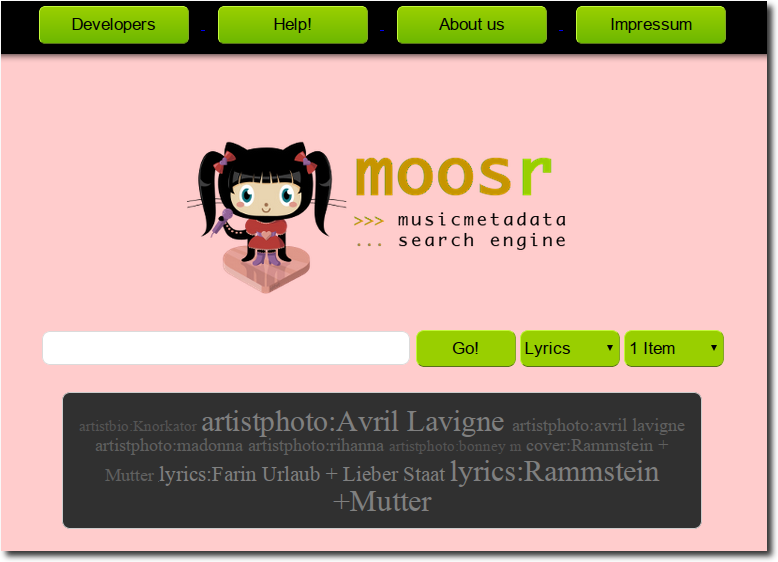
\includegraphics[scale=0.5]{../screenshots/old_site.png}
\end{center}


\section{Implementierung}

In Kapitel 6 (Siehe \ref{konzept_web}) sind bereits viele technische Details erläutert.

\paragraph{Tagcloud}
Die implementierte Tagcloud holt sich immer aus der Datenbank die zu einem
bestimmten Zeipunkt am meist gesuchten Schlagwörter raus. Dadurch wird die
Linkkraft auf bestimmten Ergebnisse dynamisch angepasst wodurch möglicherweise
Google-User die nach diesem aktuell populären Ergebnis googlen auf unsere Seite
geleitet werden.
